%********************************************************************************
% Title: Performance Modeling of a Fog Computing System
%
% Series: Courseworks in Performance Modeling of Computer Systems and Networks
%
% Author: Giacomo Marciani <mgiacomo@amazon.com>
%
% Institution: Department of Civil Engineering and Computer Science Engineering,
% University of Rome Tor Vergata, Italy
%
% Style: ACM ART SIGCONFS (based on ACM Large v1.7)
%*******************************************************************************

\documentclass[sigconf]{acmart}

\usepackage[utf8]{inputenc}
\usepackage{booktabs}
\usepackage{algorithm2e}
\usepackage{listings}
\usepackage{color, soul}
\usepackage{graphicx}
\usepackage{lipsum}
\usepackage{epstopdf}
\usepackage{subfig}
\usepackage{bm}
\usepackage{url}
\usepackage{array}

%*******************************************************************************
% Packages setting
%*******************************************************************************
\graphicspath{{fig/}}

%*******************************************************************************
% Shared Affiliation format
%*******************************************************************************
\def\sharedaffiliation{%
\end{tabular}
\begin{tabular}{c}}

%*******************************************************************************
% Fonts
%*******************************************************************************
%\newfont{\eaddfntresz}{phvr8t at 11pt}

%*******************************************************************************
% Margins
%*******************************************************************************
%\clubpenalty=10000
%\widowpenalty=10000

%*******************************************************************************
% hyphenation
%*******************************************************************************
\hyphenation{sched-uler par-a-digm adopt-ed evolv-ing th}

%*******************************************************************************
% pseudocode customisation
%*******************************************************************************
%\makeatletter
%\def\BState{\State\hskip-\ALG@thistlm}
%\makeatother

%*******************************************************************************
% Details
%*******************************************************************************
\acmConference[PMCSN'20]{Performance Modeling of a Fog Computing System}{February 2021}{Rome, Italy}
\acmYear{2021}
\copyrightyear{2021}
\setcopyright{rightsretained}
\acmISBN{123-4567-24-567/08/06}
\acmDOI{10.475/123_4}
\acmPrice{15.00}

\begin{document}
%*******************************************************************************
% Title
%*******************************************************************************
\title{Performance Modeling of a Fog Computing System}

%*******************************************************************************
% Authors
%*******************************************************************************
\author{Giacomo Marciani}
\orcid{0000-0002-3675-8804}
\affiliation{%
  \institution{University of Rome Tor Vergata}
  \streetaddress{Via del Politecnico 1}
  \city{Rome}
  \state{Italy}
  \postcode{00133}
}
\email{mgiacomo@amazon.com}

\renewcommand{\shortauthors}{G. Marciani}

%*******************************************************************************
% Contents
%*******************************************************************************
% From mitthesis package
% Version: 1.01, 2023/06/19
% Documentation: https://ctan.org/pkg/mitthesis
%
% The abstract environment creates all the required headers and footnote. 
% You only need to add the text of the abstract itself.
%
% Approximately 500 words or less; try not to use formulas or special characters
% If you don't want an initial indentation, do \noindent at the start of the abstract

The developments of the ``kinetic theory'' of gases made within the last ten years have enabled it to account satisfactorily for many of the laws of gases. The mathematical deductions of Clausius, Maxwell and others, based upon the hypothesis of a gas composed of molecules acting upon each other at impact like perfectly elastic spheres, have furnished expressions for the laws of its elasticity, viscosity, conductivity for heat, diffusive power and other properties. For some of these laws we have experimental data of value in testing the validity of these deductions and assumptions. Next to the elasticity, perhaps the phenomena of the viscosity of gases are best adapted to investigation.\footnote{Text from Holman (1876): \doi{10.2307/25138434}.}  

% http://dl.acm.org/ccs.cfm

\begin{CCSXML}
    <ccs2012>
    <concept>
        <concept_id>10002944.10011122.10002945</concept_id>
        <concept_desc>General and reference~Surveys and overviews</concept_desc>
        <concept_significance>500</concept_significance>
    </concept>
    <concept>
        <concept_id>10002978</concept_id>
        <concept_desc>Security and privacy</concept_desc>
        <concept_significance>500</concept_significance>
    </concept>
    <concept>
        <concept_id>10002978.10003022</concept_id>
        <concept_desc>Security and privacy~Software and application security</concept_desc>
        <concept_significance>500</concept_significance>
    </concept>
    </ccs2012>
\end{CCSXML}

\ccsdesc[500]{General and reference~Surveys and overviews}
\ccsdesc[500]{Security and privacy~Software and application security}

\keywords{computer security; botnet}

\maketitle
\chapter{Introduction}
\label{chp:introduction}


% %
% HEADER
% %
INSERT HERE AN EXPANSION OF THE ABSTRACT


% %
% RELATED WORKS
% %
Elasticity is a key feature for DSP systems that is attracting many research efforts. 
%
Most approaches that enable elasticity exploit best-effort threshold-based policies based on the utilization of either the system nodes or the operational abstraction, e.g. containers or data stream processing operators.
%
Other works, e.g., [1,2,8], use more complex policies to determine the scaling decisions, exploiting optimization theory [1], control theory [2], or queueing theory [8].

To the best of our knowledge, only one
work [5] has so far exploited RL techniques to drive the auto-scaling decisions in
DSP systems. Heinze et al. [5] propose a simple RL approach that learns from
experience when to acquire and release computing nodes so to efficiently process
the incoming workload. The per-operator auto-scaler populates a lookup table
that associates the utilization of the node on which the operator is executed with
the action to perform (i.e., scale in, scale out, or do nothing). The adaptation
goal is to keep the system utilization within a specific range; the SARSA learning
algorithm [12] is used to update the lookup table.

A larger number of works has exploited RL techniques to drive elasticity in
the Cloud computing context, as surveyed in [9]. Most of them use the simple Q-
learning RL algorithm (described in Sec. 5), which suffers from slow convergence,
as we also show in Section 6. Tesauro et al. [13] observe that RL approaches
can suffer from poor scalability in systems with a large state space, because
the lookup table has to store a separate value for every possible state-action
pair. Moreover, the performance obtained during the on-line training may be
unacceptably poor, due to the absence of domain knowledge or good heuristics.
To overcome these issues, they combine RL with a model of the system, defined
using queuing theory, which computes the initial deployment decisions and drives
the exploration actions. They use the SARSA learning algorithm, which however
suffers from slow convergence as Q-learning.

The goal of the Operator Manager is to take scaling decisions as to minimize
a long-term cost function which accounts for the operator downtime and for the
monetary cost to run the operator. The latter comprises: (i) the cost for running
the number of instances during the next time slot, and (ii) possibly a penalty
in case of SLA violation. In particular, we consider a constraint on the operator
response time, so that a penalty is paid every time the response time exceeds a
given threshold T SLA.

Since decisions are taken periodically, we consider a slotted time system with
fixed-length time intervals of length ∆t, with the i-th time slot corresponding
to the time interval [i∆t, (i + 1)∆t] (see Fig. 2). We denote by k i the number
of parallel instances at the beginning of slot i, and by λ i the average tuple rate
during slot i − 1 (the previous slot). At the beginning of slot i the Operator-
Manager makes the decision a i on whether modify or keep the current instance
configuration.


% %
% REMAINDER
% %
The remainder of this thesis is organized as follows.
%
In Chapter~\ref{chp:elasticity} we introduce the context of containers orchestrations, thus focusing on resource management, containerization and elasticity.
%
In Chapter~\ref{chp:reinforcement-learning} we give the necessary background notions about reinforcement learning, focusing on the Q-Learning technique and its comparison with respect to other techniques.
%
In Chapter~\ref{chp:kubernetes} we describe the technological environment of our work, that is focused on Kubernetes. In particular we describe its architecture and how it implements elasticity.
%
In Chapter~\ref{chp:smart-elasticity} we introduce the concept of smart elasticity, showing how we implemented it leveraging Q-Learning as an auto-scaling service in the Kuberntes anvironment.
%
In Chapter~\ref{chp:evaluation} we show the experimental results of the proposed smart elasticity technique.
%
In Chapter~\ref{chp:conclusions} we sum up our work, giving its conclusions and pointing out some promising future improvements.

\section{Goals and Objectives}
\label{sec:performance-modeling-goals-and-objectives}
\textit{Performance modeling} is the art of studying the behavior of a system in terms of performance metrics in order to maximize the return on tech investments.
To this aim, the \textit{simulation} is the most effective and scalable way to gather system insights and prove performance conjectures without even requiring the existence of the real system.

In this paper, we consider the system architecture in Figure~\ref{fig:system-architecture} and use a simulator to study its behavior with the goal of minimizing the response time.

The system is made of two following layers and accepts classed end-user workloads:

\begin{itemize}
		\item \textbf{Cloudlet:} upfront layer made of one-hop finite resources, having the ability to off-load tasks to the Cloud server, accordingly to an \textit{off-loading policy} based on the occupancy state of the Cloudlet. In particular, the Cloudlet may \textit{forward} incoming tasks to Cloud or \textit{restart} preempted tasks in Cloud with some \textit{overhead}. 
		
		\item \textbf{Cloud:} backfront layer made of a remote Cloud server with virtually unlimited resources.
\end{itemize}

We assume the Cloudlet  providing tasks with higher service rates than the Cloud because, since the former is placed on the network edge, it has lower transmission time and it is less exposed to network latencies.

We propose to evaluate the system behavior with two alternative off-loading policies:

\begin{itemize}
	\item \textbf{Off-Loading Policy 1:} the Cloudlet makes no distinction between tasks; it forwards incoming tasks to the Cloud when it has no available resources.
	
	\item \textbf{Off-Loading Policy 2:} the Cloudlet gives higher priority to $1^{st}$ class tasks; it interrupts $2^{nd}$ class tasks to free up resources for $1^{st}$ class tasks according to a thresholded occupancy level and forwards incoming tasks to the Cloud when it has no available resources.
\end{itemize}

We propose to evaluate system stationary and the following performance metrics with a $95\%$ level of confidence:

\begin{itemize}
	\item \textit{System/Cloudlet/Cloud response time} both global and per-class;
	
	\item \textit{System/Cloudlet/Cloud throughput} both global and per-class;
	
	\item \textit{System/Cloudlet/Cloud mean population} both global and per-class;
	
	\item \textit{Cloudlet interruption percentage} of the $2^{nd}$ class tasks;
	
	\item \textit{System response time of interrupted tasks}.
\end{itemize}

\begin{figure}
	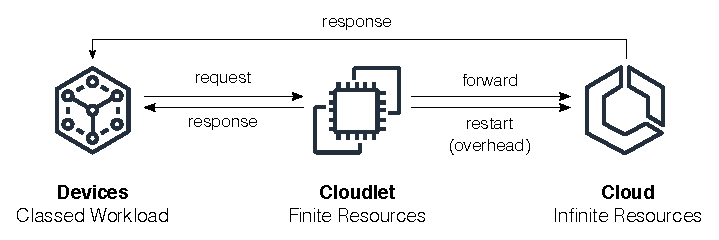
\includegraphics[width=\columnwidth]{fig/architecture}
	\caption{System architecture.}
	\label{fig:system-architecture}
\end{figure}

It is worth studying such a system because it represents the simplest form of a Fog Computing infrastructure, where the end-user workload is  served by Edge compute nodes,  possibly off-loading it to a Cloud provider. The goal of such a study is then to asses the impact of distinct off-loading policies given the trade-off between (i) Edge compute nodes, which are barely exposed to network latencies, but hardly scale and (ii) Cloud compute nodes,  which are virtually infinite, but more exposed to network latencies.
\section{Conceptual Model}
\label{sec:performance-modeling-conceptual-model}
A conceptual model defines the target system in terms of 
(i) the states it can assume over time, 
(ii) the events that let it change in time and
(iii) system assumptions.

We consider the conceptual model depicted in Figure~\ref{fig:conceptual-model-1} and \ref{fig:conceptual-model-2}, respectively for the system running the off-loading algorithm 1 and 2.
In both models, we introduced the \textit{Controller (CTRL)} component within the Cloudlet to represent the decision process of the off-loading policy.

\begin{figure}
	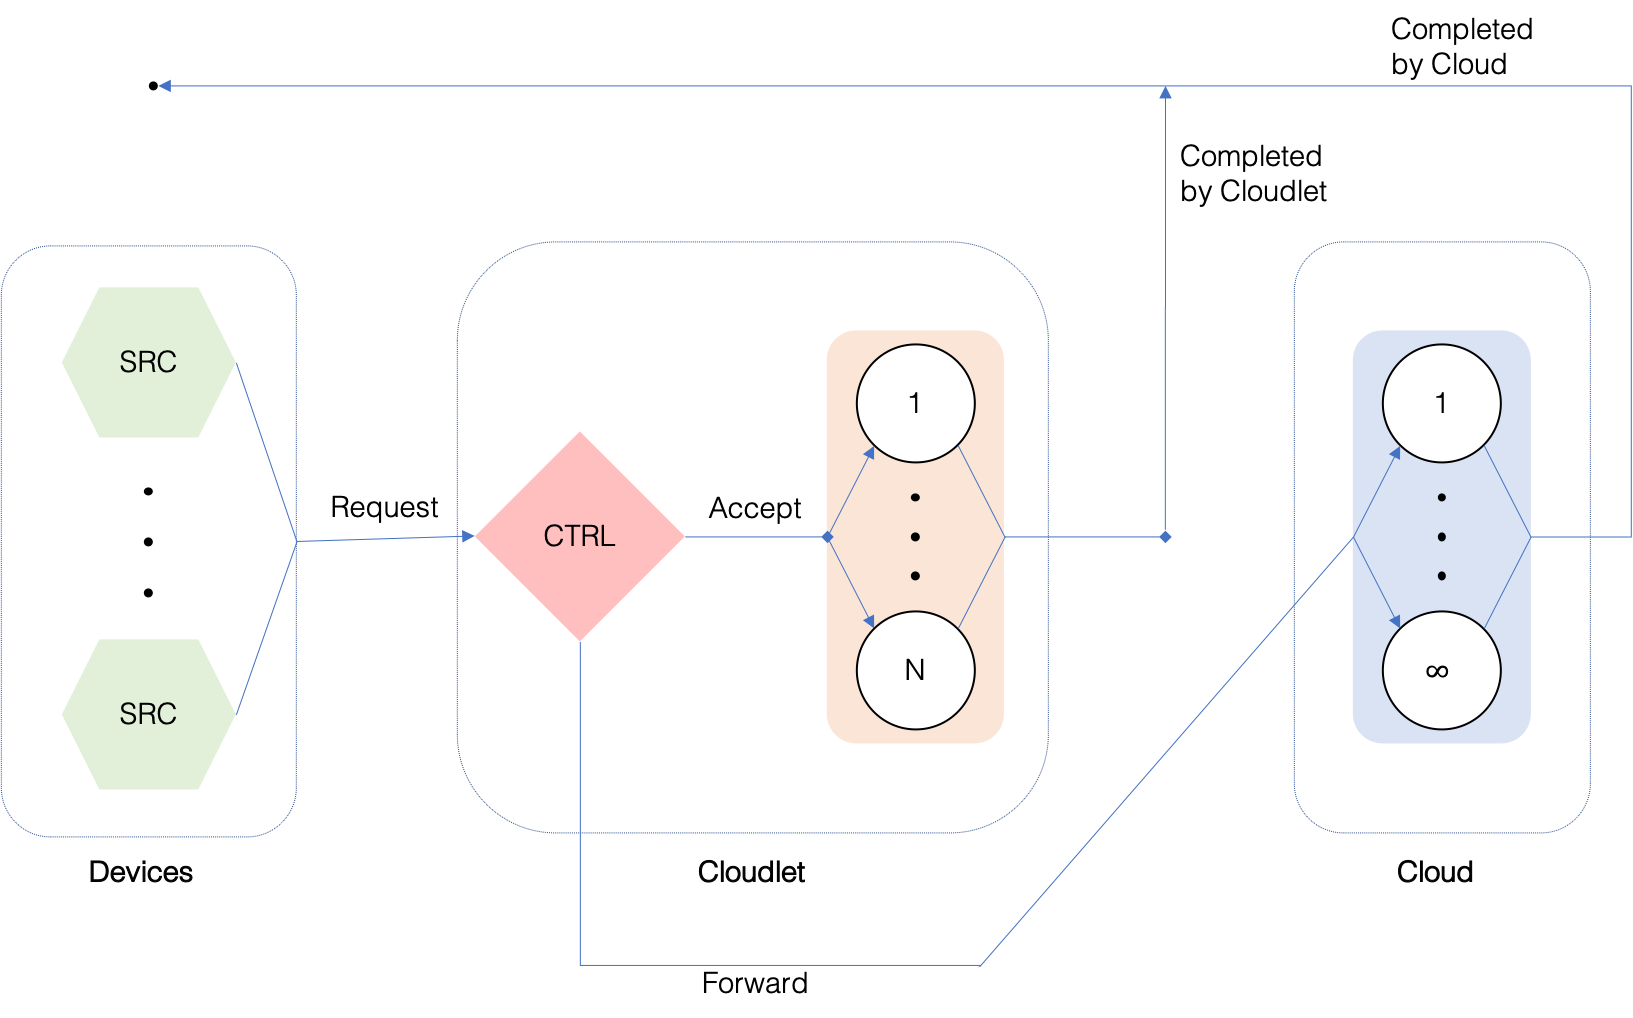
\includegraphics[width=\columnwidth]{fig/conceptual-model-1}
	\caption{Conceptual model (Off-Loading Algorithm 1).}
	\label{fig:conceptual-model-1}
\end{figure}

\begin{figure}
	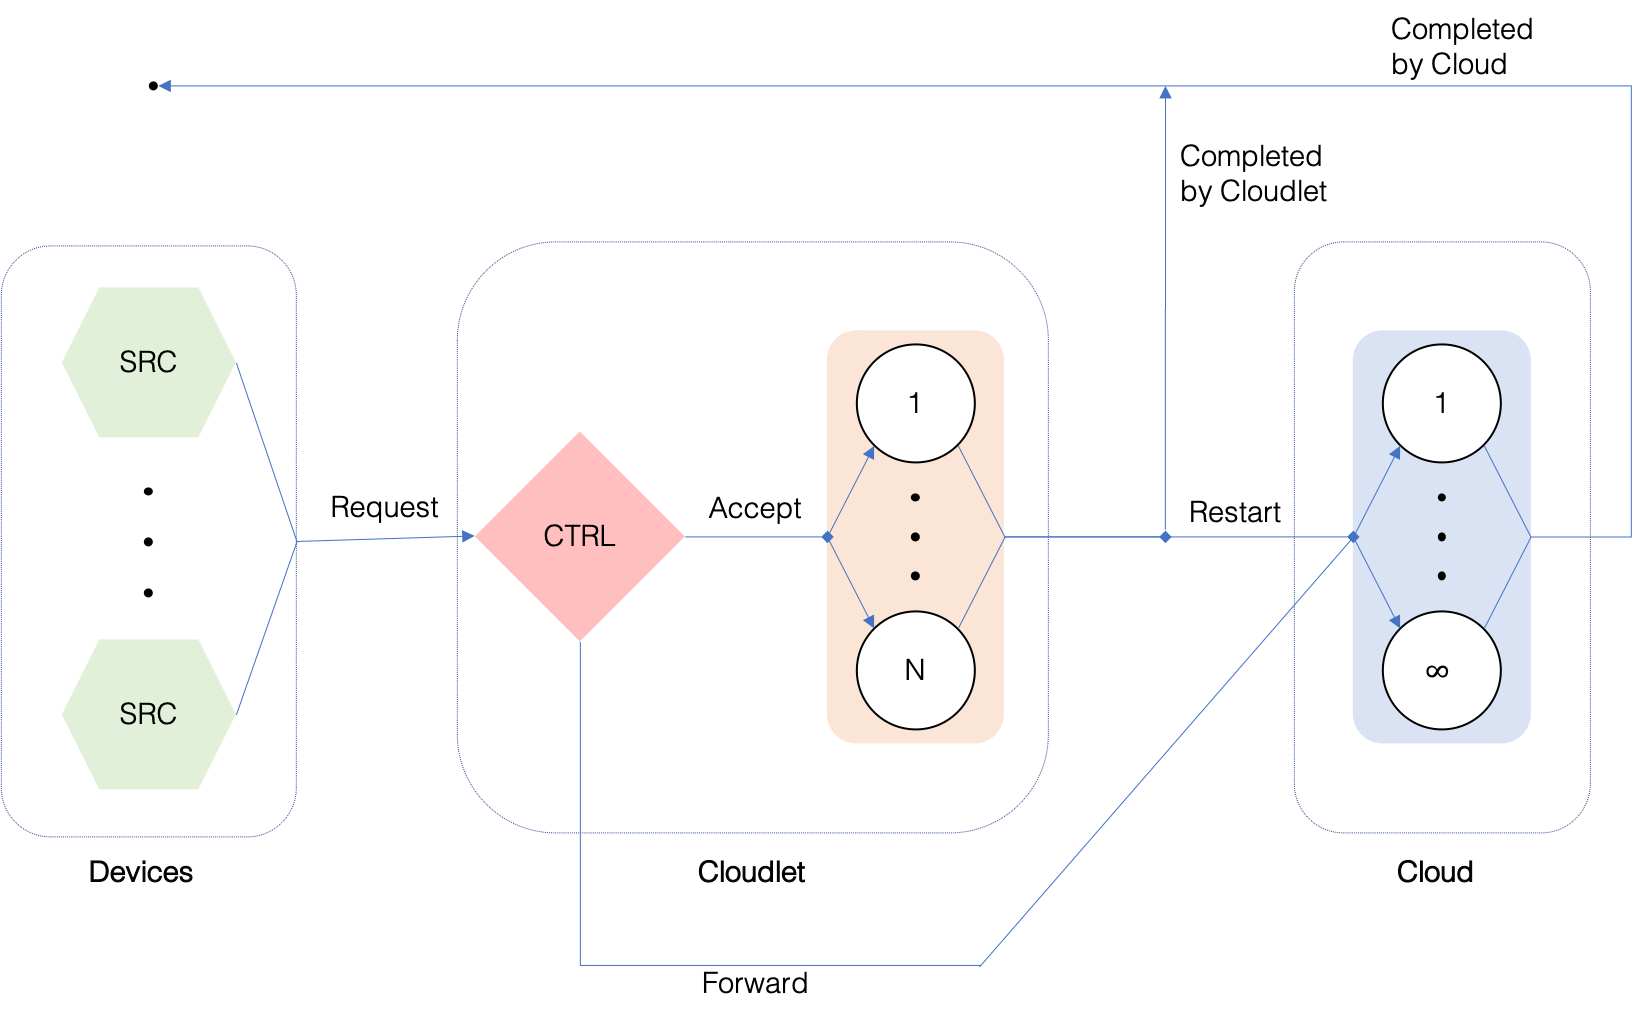
\includegraphics[width=\columnwidth]{fig/conceptual-model-2}
	\caption{Conceptual model (Off-Loading Algorithm 2).}
	\label{fig:conceptual-model-2}
\end{figure}

\paragraph{State space}
The state space $S$ of a system is a comprehensive characterization of the system at any given time.
The state space of the whole system is represented by the state space of its subsystems:

\begin{itemize}
	\item \textbf{Cloudlet}: $S_{clt} := \{(n_{clt,1},n_{clt,2})\in \mathcal{N}^{2}: n_{clt,1}+n_{clt,2}\leq N\}$, where $n_{clt,i}$ is the population of tasks belonging to the $i$-th class within the Cloudlet.
	
	\item \textbf{Cloud}: $S_{cld} := \{(n_{cld,1},n_{cld,2})\in \mathcal{N}^{2}\}$, where $n_{cld,i}$ is the population of tasks belonging to the $i$-th class within the Cloud.
\end{itemize}

\paragraph{Events space}
An event is an occurrence that could change the state of the system at the event time, according to the event type.
We consider the following events:

\begin{itemize}
	\item \textbf{arrival event $A_{clt,i}$:} a task belonging to the $i$-th class arrives to the Cloudlet.
	
	\item \textbf{arrival event $A_{cld,i}$:} a task belonging to the $i$-th class arrives to the Cloud.

	\item \textbf{completion event $C_{clt,i}$:}  a task belonging to the $i$-th class is completed by the Cloudlet.
	
	\item \textbf{completion event $C_{cld,i}$:}  a task belonging to the $i$-th class is completed by the Cloud.
	
	\item \textbf{interruption event $I_{i}$:} a task belonging to the $i$-th class is interrupted in the Cloudlet and restarted in the Cloud\footnote{notice that the interruption event is possible only for $2^{nd}$ class tasks when the Off-Loading Policy 2 is adopted.}.
\end{itemize}

\paragraph{Assumptions}
The following assumptions hold for the modeled system and ensure that we can adopt the \textit{Next-Event Simulation Model}.

\begin{itemize}
	\item \textbf{Stochastic:} the system behavior is driven by some random components, such as task arrivals and service times.
	
	\item \textbf{Dynamic:} the state of the system evolves with the time during a finite observation period. Notice that even if this period may be long enough to reach a steady state, it is finite anyway.
	
	\item \textbf{Discrete:} the state of the system evolves as a step-wise function. Notice that this assumption holds because the state space is in $\mathcal{N}^{i}$ for some $i$ and the time of events is in $\mathcal{N}$.
	
	\item \textbf{Conservative:} it is not possible to have idle resources as long as there are unprocessed tasks; alternatively speaking, as soon as a resource completes the service for a task, it immediately starts with the next eligible task (if any), with no idle time in between.
	
	\item \textbf{Flow Balanced:} the number of completed tasks is equal to the number of  arrived tasks in the observation period; alternatively speaking, given an observation period, every task that arrives to the system, it is served by the system within the same period. This assumption may sounds unacceptable given that the Cloudlet may reject some tasks, but it holds anyway because such tasks are not dropped but sent to the Cloud that, having infinite resources, always guarantees them to be served.
\end{itemize}
\section{Specification Model}
\label{sec:performance-modeling-specification-model}
The typical modeling workflow requires to specify
(i) the statistical analysis of data collected from the real system in order to determine the input model to drive simulations,
(ii) the analytical model and equations to determine performance metrics,
(iii) the adopted simulation approach and
(iv) the algorithms involved in computations.

\paragraph{Statistical specifications}
We have been provided with the statistical characterization of the target system.
Tasks belonging to the $i$-th class arrive to the system according to an exponential arrival process with rate $ \lambda_{i}$.
The Cloudlet serves tasks belonging to the $i$-th class according to an exponential service process with rate $\mu_{clt,i}$.
The Cloud serves tasks belonging to the $i$-th class according to an exponential service process with rate $\mu_{cld,i}$.
We assume that 
(i) $\mu_{clt,i}>\mu_{cld,i}\ \forall i=1,2$ and
(ii) the setup time $T_{setup}$ is exponentially distributed with expected value $E[T_{setup}]$.

In particular, we consider values shown in Equations~\ref{eqn:statistical-specifications}.

\begin{equation} 
\begin{split}
\lambda_{1}  &=6.00\;tasks/sec \\
\lambda_{2}  &=6.25\;tasks/sec \\
\mu_{clt,1}  &=0.45\;tasks/sec \\
\mu_{clt,2}  &=0.27\;tasks/sec \\
\mu_{cld,1}  &=0.25\;tasks/sec \\
\mu_{cld,2}  &=0.22\;tasks/sec \\
E[T_{setup}] &=0.8\;sec \\
\end{split}
\label{eqn:statistical-specifications}
\end{equation}

\paragraph{Analytical Model}
Given the importance and complexity of the analytical model, we preferred to reserve the whole Section~\ref{sec:analytical-model} to present it.

\paragraph{Simulation Approach}
We decided to adopt the \textit{next-event simulation method}, which is the most effective discrete-event technique in terms of algorithmic modeling, time management and computational requirements.

\paragraph{Algorithmic specifications}
From the point of view of algorithms involved in the simulation, we need to specify:

\begin{itemize}
	
	\item \textit{Off-Loading Algorithm}: defines the off-loading policy implemented by the \textit{Cloudlet Controller (CTRL)}.
	%
	The first policy, defined in Algorithm~\ref{alg:off-loading-policy-1}, makes no distinction between classes of tasks, which are all served by the Cloudlet as long as it has available resources. 
	%
	The second policy, defined in Algorithm~\ref{alg:off-loading-policy-2}, gives higher priority to the $1^{st}$ class tasks by 
	(i) accepting in Cloudlet at most $S$ $2^{nd}$ class tasks and 
	(ii) freeing up Cloudlet resources occupied by the $2^{nd}$ class tasks in favor of $1^{st}$ class tasks restarting the former on Cloud.
	Notice that the threshold $S$ plays a key role here.
	On one hand, a high $S$ increases the opportunity for  $2^{nd}$ class tasks to be served by the Cloudlet, that is faster than the Cloud.
	On the other hand, a high $S$ increases also the risk for $2^{nd}$ class tasks to incur in the overhead caused by the restart in Cloud.
	
	\item \textit{Simulation Algorithm}: defines the main execution flow of the simulator, as specified in Algorithm~\ref{alg:simulation-workflow}.
\end{itemize}

With reference to the simulation algorithm, it is worth focusing on the following aspects:

\begin{itemize}
	
	\item \textit{event generation}: a new \textit{arrival event} is generated every time an arrival is processed and the closed-door condition does not hold. We adopted Algorithm~\ref{alg:arrivals} to generate classed arrivals, whose statistical correctness relies on the properties of the exponential distribution.
	%
	A new \textit{completion event} is generated every time an arrival is processed.
	%
	A new \textit{interruption event} is generated when an arrival is processed and the Cloudlet Controller determines that a task must be interrupted in the Cloudlet and restarted in the Cloud~\footnote{the generation of interruption events is possible only when Off-Loading Policy 2 is adopted.}.
	%
	Notice that the interruption event is never mentioned in the simulation workflow in Algorithm~\ref{alg:simulation-workflow}; this is because the interruption event is not an external arrival, but an internal task switching between subsystems.
	
	\item \textit{event submission}: when a new event is submitted to the system, the simulator updates (i) the system state and (ii) the simulation counters, e.g. number of arrivals, number of completions and so on.
	
	\item \textit{closed-door condition}: when this condition holds true, no more arrivals will be generated and system will only handle remaining completion events until it reaches the idle state. 
	This condition is crucial because it identifies the point in time when the simulator has collected enough data to achieve our goals. 
	To this aim, this condition holds true when the simulator has collected the configured number of batches, i.e. 64 batches with 512 samples each.
	
	\item \textit{stop condition}: when this condition holds true, the simulation is terminated. The logical definition of this condition depends on whether the simulator is used for the performance analysis in the transient state or in the steady state.
	
	In transient analysis, the condition holds true when the simulation clock is greater than a given stop time because we want to study whether or not performance metrics to converge to stable values within the given amount of time.
	
	In performance analysis, the condition holds true when the closed-door condition does and the system has reached the idle state because we assume that the steady state exists and we want to collect enough data to generated meaningful confidence intervals.
	
	\item \textit{sampling condition}: when this condition holds true, performance metrics should be sampled. 
	In particular, it holds true when the processed event is a completion. 
	We did like this because 
	(i) sampling, as any other operation within the simulator, should happen in correspondence of an event, by design, and
	(ii) a completion events brings a super set of insights w.r.t. an arrival.
	
	
	\item \textit{metrics management}: when an event is submitted to the system, all the simulation counters are updated, e.g. number of arrivals, service time, integral areas and so on. 
	When the sampling condition holds true, those counters are used to compute a sample of performance metrics. Such a sample is then used to update performance statistics leveraging \textit{One-Pass Wellford algorithm, batch means and confidence intervals} with formulas and algorithms described in \cite{leemis2006discrete}.
	
	We decoupled counters updates and metrics sampling in this way in order to improve the simulator performances both in terms of timing and memory consumption.
	%
	In fact
	(i) the former is a low-effort operation that must be executed whenever a new event is processed,
	(ii) the latter is a higher-effort operation that should be executed in correspondence of the event type carrying the most complete set of information, i.e. completion events.
	%
	Furthermore, we preferred to compute metrics by executing metrics updates within the simulation loop rather than at the end of the simulation because in this way we can consume subsets of data points at every sampling operation rather than collecting all of them until the end, thus saving up memory.
\end{itemize}

\begin{algorithm}
	\SetAlgoLined
	\If{arrival of class 1 or class 2}{
		\eIf{$n_{clt,1}+n_{clt,2}=N$}{
			send to the Cloud
		}{
			accept on Cloudlet
		}
	}
	\caption{Off-Loading Policy 1 (OP1).}
	\label{alg:off-loading-policy-1}
\end{algorithm}

\begin{algorithm}
	\SetAlgoLined
	\If{arrival of class 1}{
		\If{$n_{clt,1}=N$}{
			send to the Cloud
		} 
		\If{$n_{clt,1}+n_{clt,2}<S$}{
			accept on the Cloudlet
		} 
		\eIf{$n_{clt,2} > 0$}{
			accept on the Cloudlet, interrupt a $2^{nd}$ class task in the Cloudlet and restart it in the Cloud
		}{
			accept on Cloudlet
		}
	}
	\If{arrival of class 2}{
		\eIf{$n_{clt,1}+n_{clt,2}>=S$}{
			send to the Cloud
		}{
			accept on the Cloudlet
		}
	}
	\caption{Off-Loading Policy 2 (OP2).}
	\label{alg:off-loading-policy-2}
\end{algorithm}

\begin{algorithm}
	\SetAlgoLined
	
	calendar.schedule\_arrival();
	
	\While{$\neg stop\_condition()$}{
		e = calendar.next\_event();
		
		\If{$e.type = completion$}{
			submit\_event(e);
		}
	
		\If{$e.type = arrival \land \neg close\_door\_condition()$}{
			e\_next = submit\_event(e);
			
			calendar.schedule(e\_next);
			
			calendar.schedule\_arrival();
		}
	
		update\_simulation\_counters();

		\If{$sampling\_condition()$}{
			sample = sampling();
			
			update\_metrics(sample);
		}
	}

\caption{Simulation Workflow.}
\label{alg:simulation-workflow}
\end{algorithm}

\begin{algorithm}
	\SetAlgoLined
	
	rndgen.select\_stream(ARRIVAL)
	
	$p_{1}=\frac{\lambda_{1}}{\lambda_{1}+\lambda_{2}}$
	
	u = rndgen.uniform(0.0,1.0)
	
	\eIf{$u\leq p_{1}$}{
		arrival\_type = TASK\_1
		
		rndgen.select\_stream(ARRIVAL\_TASK\_1)
		
		$t_{inter-arrival}$ = rndgen.exponential($\lambda_{1}$)
	}{
		arrival\_type = TASK\_2
		
		rndgen.select\_stream(ARRIVAL\_TASK\_2)
		
		$t_{inter-arrival}$ = rndgen.exponential($\lambda_{2}$)
	}
	
	$t_{arrival}=t_{last\_arrival}+t_{inter-arrival}$

	$t_{last\_arrival}=t_{arrival}$
	
	schedule(arrival\_type,$t_{arrival}$)
	\caption{Generation of arrivals.}
	\label{alg:arrivals}
\end{algorithm}


\section{Computational Model}
\label{sec:performance-modeling-computational-model}
The simulator has been designed following the \textit{next-event simulation} paradigm \cite{leemis2006discrete} and has been implemented as a \textit{Pythonv3.9} CLI application. 
The open source code is available in a public Github repository \cite{gmarciani-pydes}.

In this Section, we provide a short description of the simulator configurabili and the main software classes implementing the simulator, in order to help the reader go through our code.

\paragraph{Configuration}
The simulator can be fully configured with a YAML file loaded when the simulator starts up. 
In particular, the following parameters can be configured:

\begin{itemize}
	\item \textit{arrival process}: statistical distribution law and parameters of arrivals for both task classes. In this work, we considered the Exponential distribution, even if any statistical distribution can be set\footnote{Notice that, even if the simulator supports any statistical distribution for the arrival process, the generation of arrivals shown in Algorithm~\ref{alg:arrivals} and the analytical models presented in Section~\ref{sec:analytical-model} are valid only for exponential arrivals.}.
	
	\item \textit{service process}: statistical distribution law and parameters of services for both task classes. In this work, we considered the Exponential distribution, even if any statistical distribution can be set.
	
	\item \textit{setup time}: statistical distribution law and parameters of the setup time for both task classes. In this work, we considered an Exponential setup time for the $2^{nd}$ class, even if any statistical distribution can be set.
	
	\item \textit{Cloudlet dimension}: number of Cloudlet resources. In this work, we considered a dimension of $20$ resources.
	
	\item \textit{Cloudlet Controller Algorithm}: Off-Loading Policy run by the Cloudlet Controller. In this work, we considered policies shown in Section~\ref{sec:performance-modeling-specification-model}, but the simulator has been designed to be easily extended with different custom policies.
		
	\item \textit{Cloudlet threshold}: threshold for the restart condition of $2^{nd}$ class tasks in the Cloudlet\footnote{this configuration is considered by the simulator only when the Cloudlet Controller runs the Off-Loading Policy 2.}. In this work, we considered values in $[1,20]$.
	
	\item \textit{server selection}: policy adopted to select the $2^{nd}$ class task to interrupt in the Cloudlet when the threshold has been reached\footnote{this configuration is considered by the simulator only when the Cloudlet Controller runs the Off-Loading Policy 2.}. In this work, we consider the Random selection, but the user can choose among Random, Ordered, Cyclic and Equity selection policies.
\end{itemize}

\paragraph{Simulation Workflow}
The main class implementing the simulation workflow is:

\begin{itemize}
	
	\item \textit{Simulation}: simulator entry-point, responsible to load configurations and drive the simulation workflow. In particular
	(i) it creates the calendar of events, the target system and statistics objects, 
	(ii) shows the real-time progress of the simulation, 
	(iii) writes raw data files and output reports.

\end{itemize}

\paragraph{Event management}
Events are managed by a \textit{priority-queue based calendar} with the ability both to schedule and un-schedule events\footnote{when a task is interrupted within the Cloudlet and restarted in the Cloud, the initial Cloud completion event is actually un-scheduled and a brand new Cloud completion event is scheduled as a replacement.}.
%
The calendar is initialized by scheduling the first arrival in the initialization phase. The submission of an arrival $a$ to the system could in fact induce
(i) the scheduling of the corresponding completion event,
(ii) the scheduling of a new arrival, or
(iii) the un-scheduling of a previously scheduled completion, i.e. interruption in Cloudlet.

The main classes implementing event management are:

\begin{itemize}
	
	\item \textit{Calendar}: calendar of events, implemented as a priority-queue with the ability to both schedule and un-schedule events.
	
\end{itemize}

\paragraph{System}
The main classes implementing the target system are:

\begin{itemize}
	
	\item \textit{System}: high level abstraction of the whole system, responsible to initialize the Cloudlet, initialize the Cloud, implement the Controller logic and update system-level classed/global metrics.
	
	\item \textit{Cloudlet}: represents the Cloudlet subsystem, responsible to handle events, select the task to interrupt according to the selection policy and update Cloudlet-level classed/global metrics.
	
	\item \textit{Cloud}: represents the Cloud subsystem, responsible to handle events and update Cloudlet-level classed/global metrics.
	
\end{itemize}

\paragraph{Randomization}
Random components are ruled by a custom \textit{multi-stream Lehmer generator} to generate pseudo-random events.
The implementation of the generator and its experimental evaluation are respectively described later on in Section~\ref{sec:random-number-generation} and Section~\ref{sec:evaluation}.
The \textit{degree of randomization} has been improved by associating the following processes to a dedicated stream of the pseudo-random number generator: type selection for the next arrival, arrival process of each task class, service process of each servant and server selection rule.
This approach has been motivated by the fact that in a real case scenario we can assume the independence between (i) inter-classed workload, (ii) computational offer of distinct resources and (iii) selection strategies.

The main classes implementing the random processes are:

\begin{itemize}
	
	\item \textit{RndGen}: instance of a fully-customizable multi-stream Lehmer pseudo-random number generator.
	
	\item \textit{RandomComponent}: represents a fully-customizable independent random process. In particular, the calendar and each subsystem receive as input an instance of this object in order to realize their own random logic.
	
\end{itemize}

\paragraph{Metrics}
The main classes implementing metrics and statistics are:

\begin{itemize}
	
	\item \textit{SimulationMetrics}: abstraction encapsulating all counters and performance metrics involved in the simulation, responsible to make it easy to update metrics during the simulation loop. In particular, each subsystem receives as input a reference to this singleton in order to decentralize and isolate the updates of metrics leveraging the well-know IoC software design pattern.
	
	\item \textit{BatchedMeasure}: an object that represents a measurement with both an instantaneous value and mean, standard deviation and confidence interval leveraging the batch means technique and the confidence interval estimation, as defined in \cite{leemis2006discrete}.
	
	\item \textit{WelfordAccumulator}: an object that is able to return in-place updated mean and standard deviation leveraging the \textit{one-pass Welford algorithm}. This object is widely adopted in our software, as it is used to update batch means.
	
	\item \textit{Sample}: an object that represents the instantaneous sample of simulation counters and performance metrics. It is used in our simulator to create a snapshot of metrics during the sampling process.
	
\end{itemize}

\paragraph{Analytical Solver}
The main classes implementing the analytical model resolution logic are:

\begin{itemize}

	\item \textit{AnalyticalSolver}: an object that is able to compute the analytical solution for the target system. In particular, this solver leverages our Markov Chain generator and an efficient symbolic solver for the resolution of flow-balance equations. The calculus of performance metrics is ruled by the same formulas specified in section dedicated to the analytical model.

\end{itemize}

\paragraph{Correctness}
The correct behavior of mission critical classes has been covered by unit testing implemented with the built-in Python testing library.
\section{Verification}
\label{sec:performance-modeling-verification}
The main goal of verification is to assess the consistency of the computational model with the specification model.
The verification has been carried out by evaluating the following consistency checks based on simulator logs and output reports:

\begin{itemize}
	\item \textbf{state consistency:} verifies the correctness of the system state evolution, i.e. given an event, it implies the expected system state transition;
	
	\item \textbf{clock consistency:} verifies the correctness of the simulation clock evolution, i.e. given an event, it implies the expected simulation clock transition;
	
	\item \textbf{arrival consistency:} verifies the correctness of arrivals ordering, i.e. given a set of tasks, they took service following the arrival order;
	
	\item \textbf{completion consistency:} verifies the correctness of completion ordering, i.e. given a set of tasks, they leave the system following the ascending ordering key $t_{arrival}+service$;
	
	\item \textbf{flow consistency:} verifies the correctness of the following flow trends:
	
	\begin{equation}
	n_{clt,i}=a_{clt,i}-c_{clt,i}-s_{clt,i}
	\end{equation}
	\begin{equation}
	n_{cld,i}=a_{cld,i}-c_{cld,i}+s_{cld,i}
	\end{equation}
	\begin{equation}
	s_{clt,i}=s_{cld,i}
	\end{equation}
	
	where 
	$n_{j,i}$ is the population in the $j$-th subsystem belonging to $i$-th class of tasks, 
	$a_{j,i}$ is the number of arrivals to the $j$-th subsystem belonging to $i$-th class of tasks,
	$c_{j,i}$ is the number of completions in the $j$-th subsystem belonging to $i$-th class of tasks
	$s_{j,i}$ is the number of switches from/to the $j$-th subsystem belonging to $i$-th class of tasks\footnote{notice that $s_{j,1}=0\forall j=1,2$, as tasks belonging to class $C1$ cannot be switched from Cloudlet to Cloud.}.
	 
	\item \textbf{workload change consistency:} verifies the correctness of performance metrics variations in response to arrival/service rates variations. For example, we verified that the following hold true:
	
	\begin{equation}
		\mu_{cld,2}^{new} > \mu_{cld,2}^{old} \Rightarrow E[T_{sys,2}]^{new} > E[T_{sys,2}]^{old}
	\end{equation}
	\\
	and
	
	\begin{equation}
	S^{new} > S^{old} \Rightarrow E[N_{cld,2}]^{new} < E[N_{cld,2}]^{old}
	\end{equation}
	\\
	where $S$ is the threshold for the off-loading algorithm 2.
\end{itemize}
\section{Validation}
\label{sec:performance-modeling-validation}
A well conducted performance modeling workflow should include a final validation step to assess the consistency of the model with the real system. 
%
As the simulation main purpose is insight, a widely adopted Turing-like technique is to place the computational model alongside with the real system and assess the consistency of performance metrics.
%
Clearly, we cannot adopt this technique because, since we do not have any real system at hand, we cannot compare the model with its real counterpart.
%
For this reason, we totally rely on the validation with respect to the analytical model.

In Figure \ref{tbl:evaluation-performance-metrics} we show the comparison between theoretical performance results, taken from the analytical model, and their experimental counterpart, taken from the simulator.
%
The results demonstrate that our simulator is a pretty reliable tool to conduct the performance analysis for the target system.
\section{Analytical Model}
\label{sec:analytical-model}
In this Section we define the analytical model of the system.
%
In particular, we will show the queue model, Markov Chain and performance metrics formulas for the system both running the Off-Loading Policy 1 and the Off-Loading Policy 2.
%
At the end, we will explain how we solved the analytical model to obtain theoretical results for the target case.

\paragraph{Queue Model}
As the system is characterized by Poisson arrivals and Exponential services, we could consider treating the queue model as a Jackson Network. 
Nevertheless, this would not be correct without a very strong assumption on the routing probabilities, In fact, a Jackson Network requires the routing probabilities  to be static, i.e. independent of the system state, and this is not the case.

So, \textit{we assume the routing probabilities to be static in order to unlock the potential of the Jackson Network in our analytical dissertation}.

In Figures~\ref{fig:analytical-model-queue-1} and \ref{fig:analytical-model-queue-2}, we show the queue models for the system with Off-Loading Policy 1 and Off-Loading Policy 2, respectively.

\begin{figure}delphi
	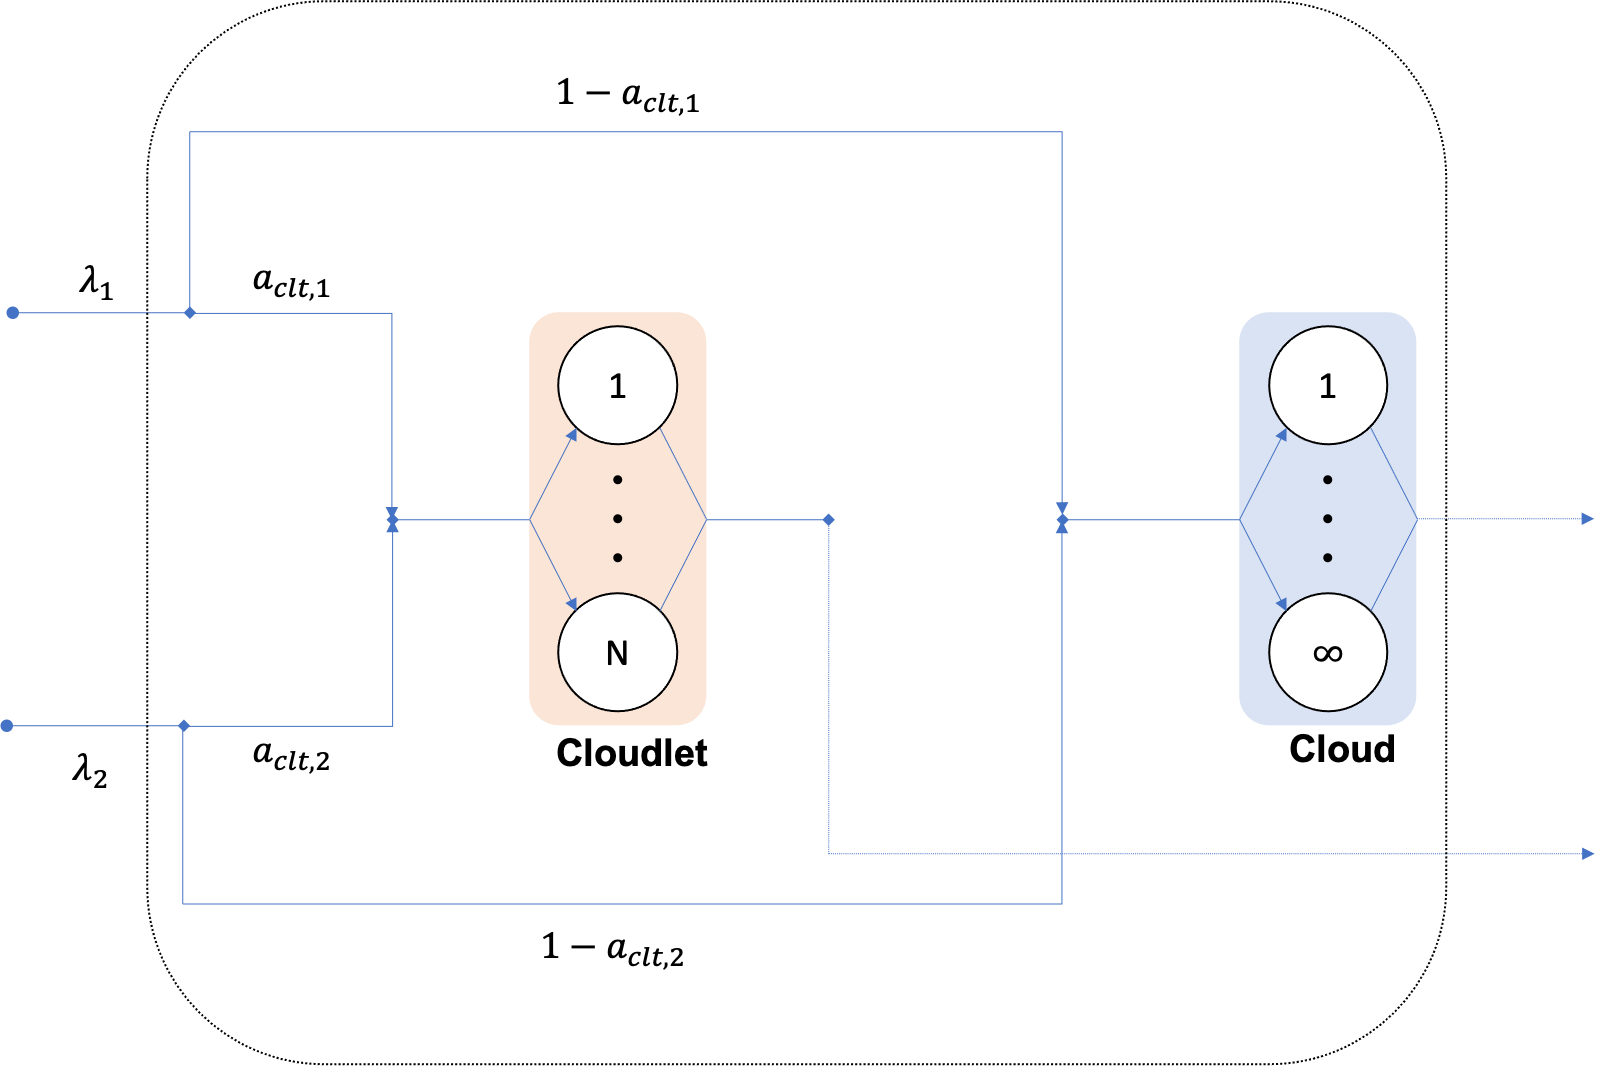
\includegraphics[width=\columnwidth]{fig/analytical-model-queue-1}
	\caption{Queue model for the system with OP1.}
	\label{fig:analytical-model-queue-1}
\end{figure}

\begin{figure}
	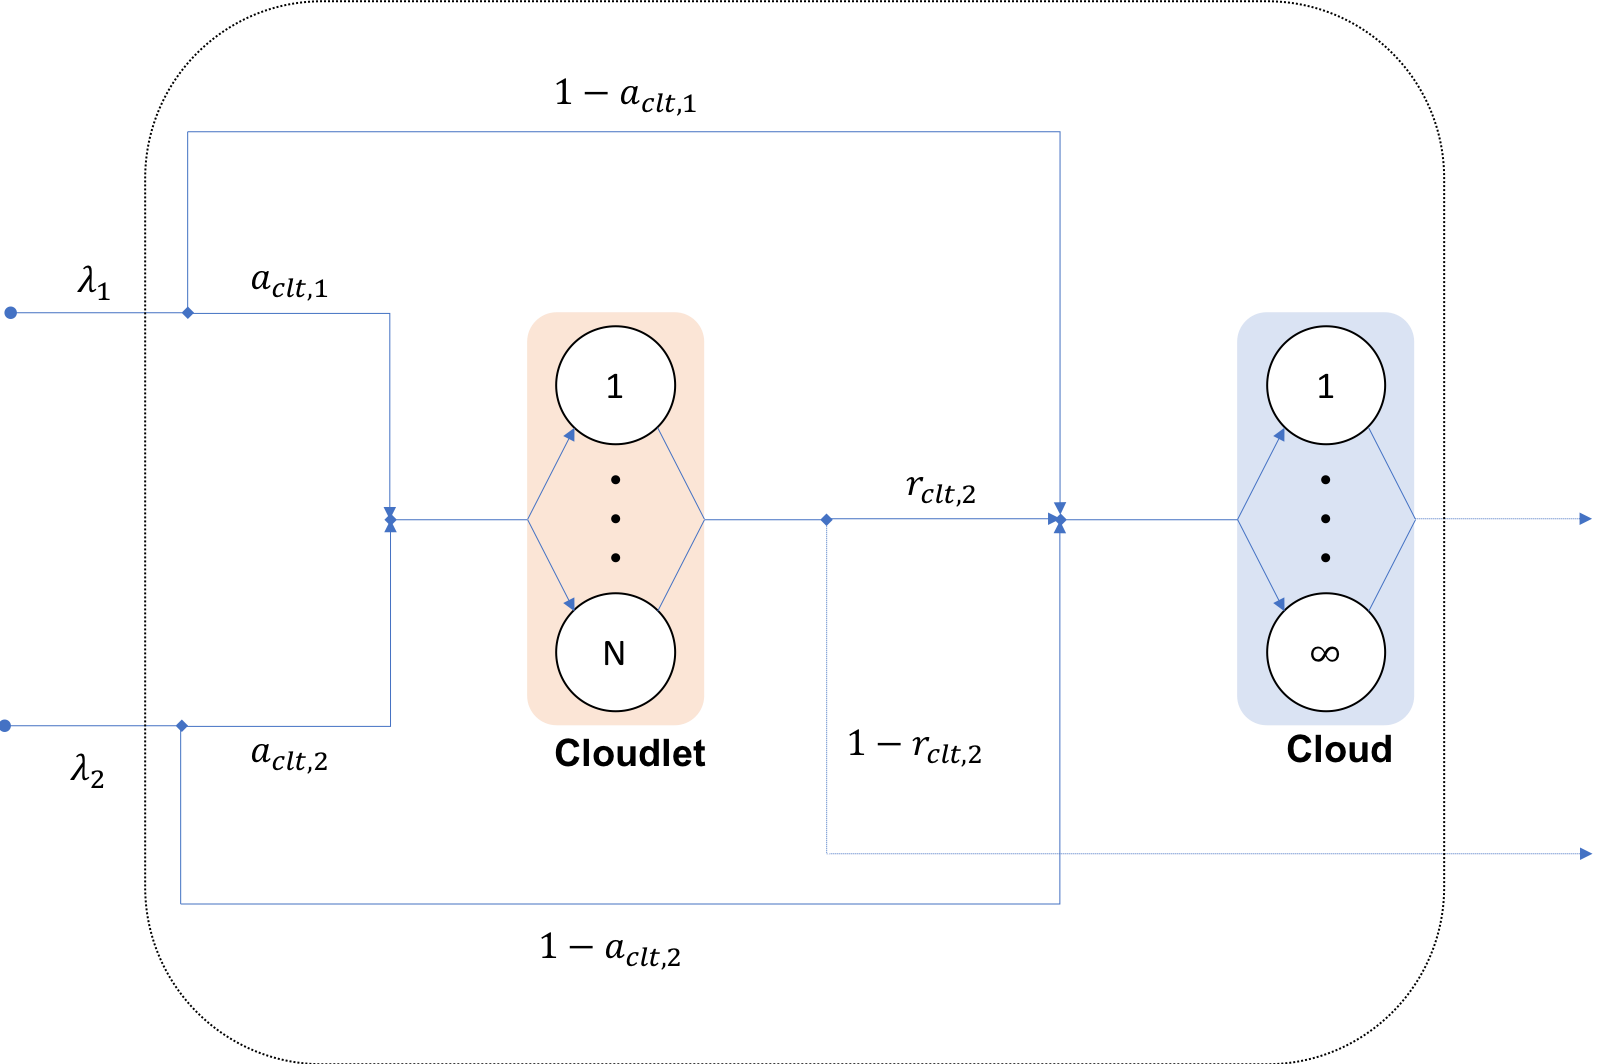
\includegraphics[width=\columnwidth]{fig/analytical-model-queue-2}
	\caption{Queue model for the system with OP2.}
	\label{fig:analytical-model-queue-2}
\end{figure}

The definition of the routing probabilities relies on the following subsets of Cloudlet states $S_{clt}$, whose definition strictly depends on the adopted off-loading policy:

\begin{itemize}
	\item $A_{clt,1}$:  subset of states where a task belonging to the $1^{st}$ class is accepted in the Cloudlet.
	
	In OP1, a $1^{st}$ class task is accepted in the Cloudlet as long as not all the $N$ resources are occupied.
	In OP2, a $1^{st}$ class task is accepted in the Cloudlet as long as not all the $N$ resources are occupied or there is at least one $2^{nd}$ class task to be interrupted.

	\begin{equation}
		A_{clt,1} :=
		\left\{
		\begin{array}{ll}
			\begin{aligned}
				& \{(n_{clt,1},n_{clt,2})\in S_{clt} : \\
				& n_{clt,1}+n_{clt,2}<N\}
			\end{aligned} & \mbox{if } OP1 \\
			\\
			\begin{aligned}
				& \{(n_{clt,1},n_{clt,2})\in S_{clt} : \\
				& n_{clt,1}+n_{clt,2}<N \vee n_{clt,2}>0\}
			\end{aligned} & \mbox{if } OP2
		\end{array}
		\right.
	\end{equation}
	
	\item $A_{clt,2}$: subset of states where  a task belonging to the $2^{nd}$ class is accepted in the Cloudlet.
	
	In OP1, a $2^{nd}$ class task is accepted in the Cloudlet as long as not all the $N$ resources are occupied.
	In OP2, a $2^{nd}$ class task is accepted in the Cloudlet as long as not all the $N$ resources are occupied and there are at most $S$ resources occupied by $2^{nd}$ class tasks.
	
	\begin{equation}
		A_{clt,2} :=
		\left\{
		\begin{array}{ll}
			\begin{aligned}
				& \{(n_{clt,1},n_{clt,2})\in S_{clt} : \\
				& n_{clt,1}+n_{clt,2}<N\}
			\end{aligned} & \mbox{if } OP1 \\
			\\
			\begin{aligned}
				& \{(n_{clt,1},n_{clt,2})\in S_{clt} : \\
				& n_{clt,1}+n_{clt,2}<N \wedge n_{clt,2}<S\}
			\end{aligned} & \mbox{if } OP2
		\end{array}
		\right.
	\end{equation}
	
	\item $R_{clt,2}$: subset of states where  a task belonging to the $2^{nd}$ class is interrupted in the Cloudlet and it is restarted in the Cloud.
	
	In OP1, the set is empty because task interruption is not provided by the policy.
	In OP2, a $2^{nd}$ class task is interrupted in the Cloudlet and restarted in the Cloud as long as the former does not have free resources and there is at least one $2^{nd}$ class task to interrupt.
	
	\begin{equation}
		R_{clt,2} :=
		\left\{
		\begin{array}{ll}
			\begin{aligned}
				& \emptyset
			\end{aligned} & \mbox{if } OP1 \\
			\\
			\begin{aligned}
				& \{(n_{clt,1},n_{clt,2})\in S_{clt} : \\
				& n_{clt,1}+n_{clt,2}=N \wedge n_{clt,2}>0\}
			\end{aligned} & \mbox{if } OP2
		\end{array}
		\right.
	\end{equation}
\end{itemize}

Given such sets, the routing probabilities  are accordingly defined:

\begin{itemize}
	
	\item $a_{clt,1}$: the probability for a demanding $1^{st}$ class task to be accepted in the Cloudlet.
	
	\begin{equation} 
		a_{clt,1} := \sum_{s\in A_{clt,1}} \pi_{s}
	\end{equation}
	
	\item $a_{clt,2}$: the probability for a demanding $2^{nd}$ class task to be accepted in the Cloudlet.
	
	\begin{equation} 
		a_{clt,2} := \sum_{s\in A_{clt,2}} \pi_{s}
	\end{equation}
		
	\item $r_{clt,2}$: the probability for a running $2^{nd}$ class task to be interrupted in the Cloudlet and restarted in the Cloud.
	
	\begin{equation} 
		\begin{split}
			r_{clt,2} & = \sum_{s\in R_{clt,2}} \pi_{s} \Big(\frac{\lambda_{1}}{\lambda_{1}+\lambda_{2}}\Big) \\
		\end{split}
	\end{equation}
\end{itemize}

\paragraph{Markov Chain}
As the system is characterized by Poisson arrivals\footnote{same as Exponential inter-arrivals.} and Exponential services, the Markovian condition holds true and we can then determine the Markov Chain\footnote{If the Markovian condition is not satisfied, Markov Chain solution must be considered only as an approximation.} whose resolution allows us to compute the routing probabilities.

For sake of simplicity, we consider here the simple case with $N=2$ in order to (i) give an idea of the system of equations to be solved and (ii) graphically recognize the critical states. 
In fact, the representation fo the Markov Chain and the associated equations would be impractical for the target case $N=20$, due to the combinatorial explosion of the state space.

In Figure~\ref{fig:analytical-model-markov-1} we show the Markov Chain for the system with Off-Loading Policy 1 and $N=2$. 
In this chain, red states represent those where both the $1^{st}$ and $2^{nd}$ class traffic is blocked by the Cloudlet and forwarded to the Cloud.
The associated flow balance equations are listed in Equation~\ref{eqn:analytical-model-markov-1}.

\begin{figure}
	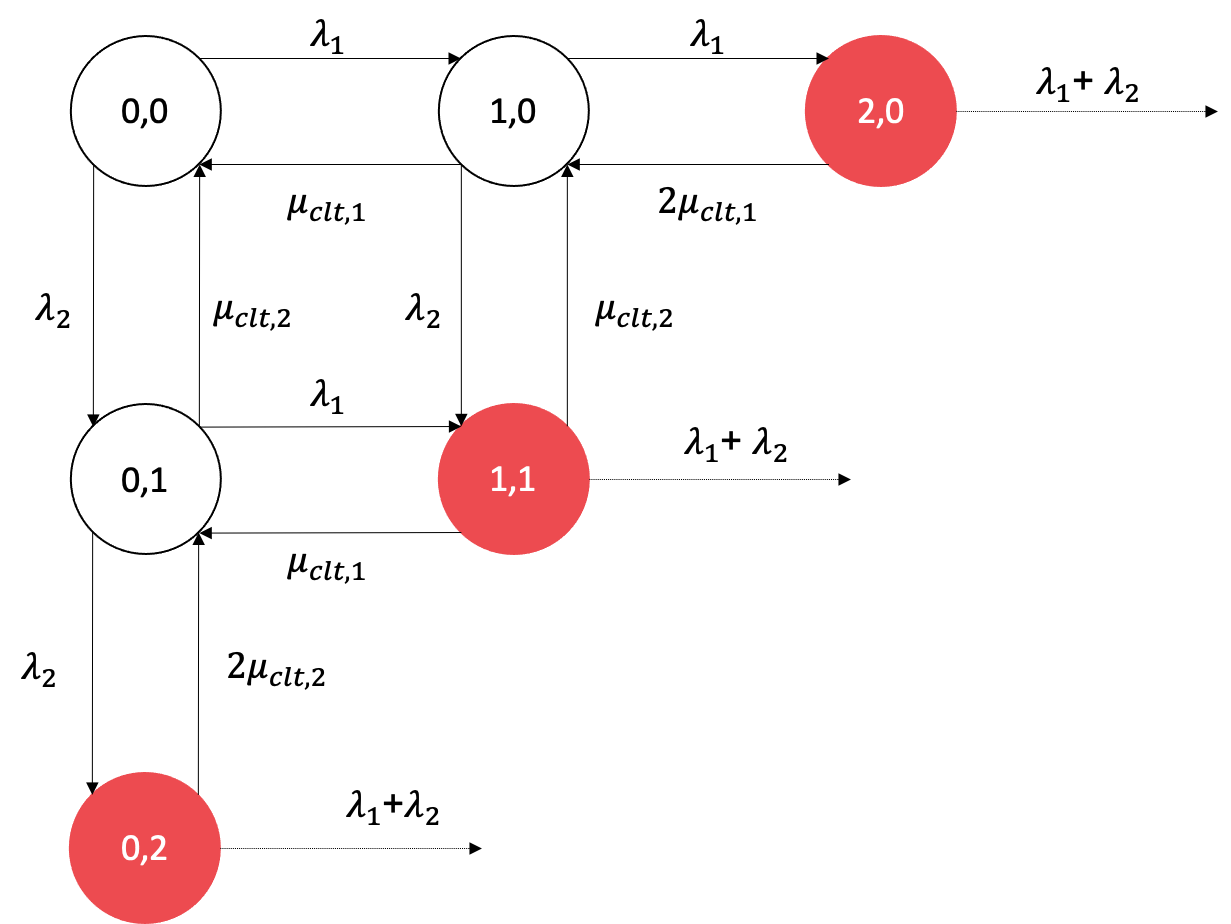
\includegraphics[width=\columnwidth]{fig/analytical-model-markov-1}
	\caption{Markov Chain for the system with OP1 (N=2).}
	\label{fig:analytical-model-markov-1}
\end{figure}

\begin{equation}
	\begin{split}
		\pi_{0,0}(\lambda_{1}+\lambda_{2})& = \pi_{1,0}\mu_{clt,1}+\pi_{0,1}\mu_{clt,2} \\
		\pi_{0,1}(\lambda_{1}+\lambda_{2}+\mu_{clt,2}) & = \pi_{0,0}\lambda_{2}+\pi_{1,1}\mu_{clt,1}+\pi_{0,2}2\mu_{clt,2} \\
		\pi_{1,0}(\lambda_{1}+\lambda_{2}+\mu_{clt,1}) & = \pi_{0,0}\lambda_{1}+\pi_{1,1}\mu_{clt,2}+\pi_{2,0}2\mu_{clt,1} \\
		\pi_{1,1}(\mu_{clt,1}+\mu_{clt,2}) & = \pi_{0,1}\lambda_{1}+\pi_{1,0}\lambda_{2} \\
		\pi_{0,2}(2\mu_{clt,2}) & = \pi_{0,1}\lambda_{2} \\
		\pi_{2,0}(2\mu_{clt,1}) & = \pi_{1,0}\lambda_{1} \\
		1 & = \pi_{0,0}+\pi_{0,1}+\pi_{1,0}+\pi_{1,1}+\pi_{0,2}+\pi_{2,0}\\
	\end{split}
	\label{eqn:analytical-model-markov-1}
\end{equation}

In Figure~\ref{fig:analytical-model-markov-2} we show the Markov Chain for the system with Off-Loading Policy 2 and $N=S=2$. 
In this chain, the red state represents the one where both the $1^{st}$ and $2^{nd}$ class traffic is blocked; whereas the orange states represent those where (i) a $1^{st}$ class arrival is accepted in Cloudlet, causing the restart in Cloud of a random running $2^{nd}$ class task and (ii) a $2^{nd}$ class arrival is blocked by the Cloudlet and forwarded to the Cloud.

\begin{figure}
	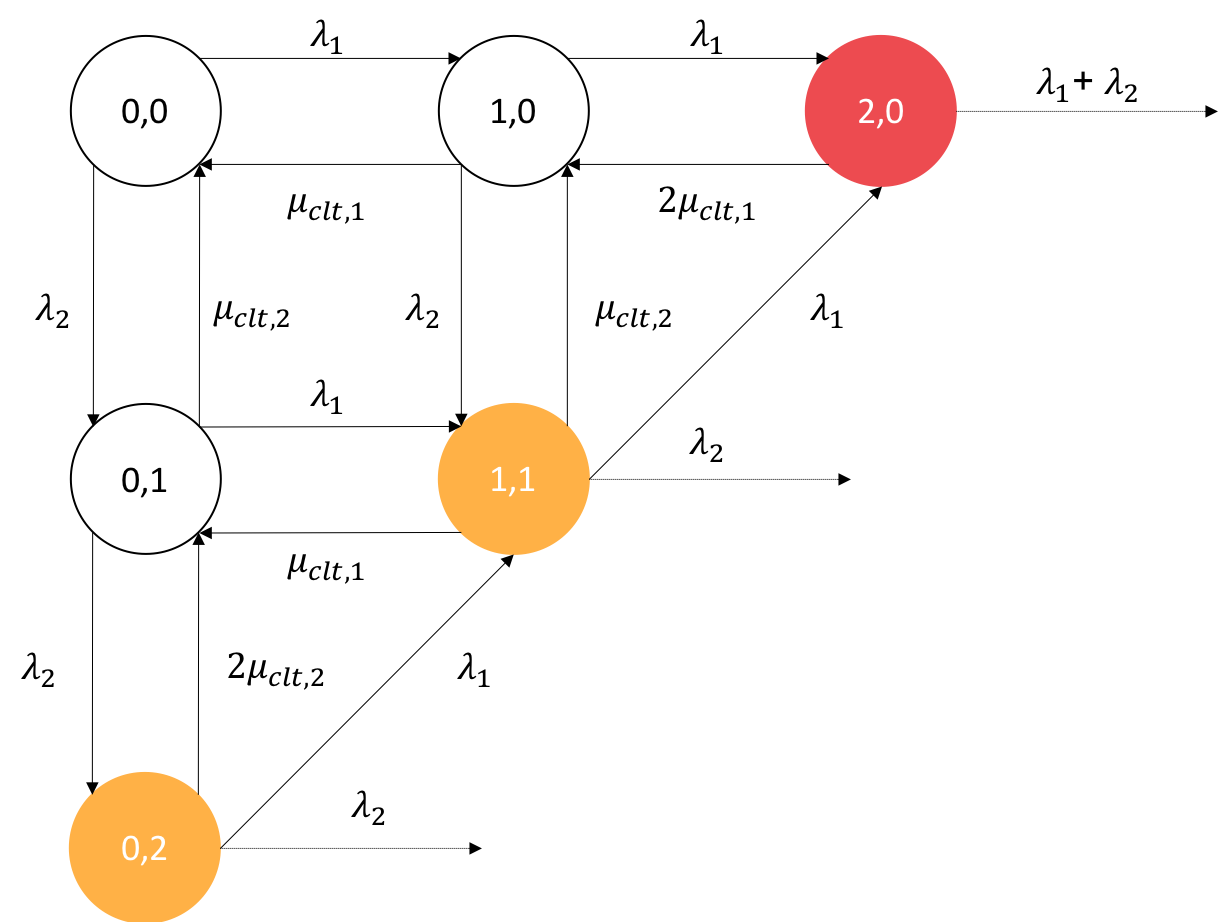
\includegraphics[width=\columnwidth]{fig/analytical-model-markov-2}
	\caption{Markov Chain for the system with OP2 (N=S=2).}
	\label{fig:analytical-model-markov-2}
\end{figure}

\begin{equation}
	\begin{split}
		\pi_{0,0}(\lambda_{1}+\lambda_{2})& = \pi_{1,0}\mu_{clt,1}+\pi_{0,1}\mu_{clt,2} \\
		\pi_{0,1}(\lambda_{1}+\lambda_{2}+\mu_{clt,2}) & = \pi_{0,0}\lambda_{2}+\pi_{1,1}\mu_{clt,1}+\pi_{0,2}2\mu_{clt,2} \\
		\pi_{1,0}(\lambda_{1}+\lambda_{2}+\mu_{clt,1}) & = \pi_{0,0}\lambda_{1}+\pi_{1,1}\mu_{clt,2}+\pi_{2,0}2\mu_{clt,1} \\
		\pi_{1,1}(\lambda_{1}+\mu_{clt,1}+\mu_{clt,2}) & = \pi_{0,1}\lambda_{1}+\pi_{1,0}\lambda_{2}+\pi_{0,2}\lambda_{1} \\
		\pi_{0,2}(\lambda_{1}+2\mu_{clt,2}) & = \pi_{0,1}\lambda_{2} \\
		\pi_{2,0}2\mu_{clt,1} & = \pi_{1,0}\lambda_{1}+\pi_{1,1}\lambda_{1} \\
		1 & = \pi_{0,0}+\pi_{0,1}+\pi_{1,0}+\pi_{1,1}+\pi_{0,2}+\pi_{2,0}\\
	\end{split}
	\label{eqn:analytical-model-markov-2}
\end{equation}

In Figure~\ref{fig:analytical-model-markov-2-1} we show the Markov Chain for the system with Off-Loading Policy 2 and $N=2,S=1$. 
In this chain, the red state represents the one where both the $1^{st}$ and $2^{nd}$ class traffic is blocked; the orange state represents the one where (i) a $1^{st}$ class arrival is accepted in Cloudlet, causing the restart in Cloud of a random running $2^{nd}$ class task and (ii) a $2^{nd}$ class arrival is blocked by the Cloudlet and forwarded to the Cloud; whereas the grey state and (ii) a $2^{nd}$ class arrival is blocked by the Cloudlet and forwarded to the Cloud.

\begin{figure}
	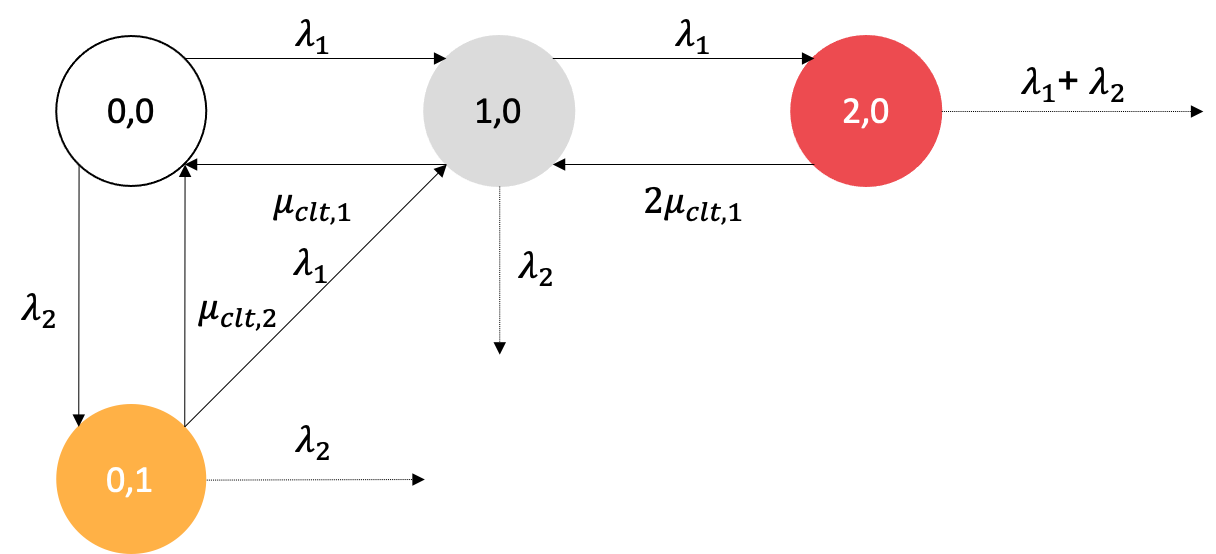
\includegraphics[width=\columnwidth]{fig/analytical-model-markov-2-1}
	\caption{Markov Chain for the system with OP2 (N=2, S=1).}
	\label{fig:analytical-model-markov-2-1}
\end{figure}

\begin{equation}
	\begin{split}
		\pi_{0,0}(\lambda_{1}+\lambda_{2})& = \pi_{1,0}\mu_{clt,1}+\pi_{0,1}\mu_{clt,2} \\
		\pi_{0,1}(\lambda_{1}+\mu_{clt,2}) & = \pi_{0,0}\lambda_{2} \\
		\pi_{1,0}(\lambda_{1}+\mu_{clt,1}) & = \pi_{0,0}\lambda_{1}+\pi_{2,0}2\mu_{clt,1} \\
		\pi_{2,0}2\mu_{clt,1} & = \pi_{1,0}\lambda_{1} \\
		1 & = \pi_{0,0}+\pi_{0,1}+\pi_{1,0}+\pi_{2,0}\\
	\end{split}
	\label{eqn:analytical-model-markov-2-1}
\end{equation}

\paragraph{Accepted Workload}
Given the routing probabilities we can determine the following accepted workloads:

\begin{itemize}
	\item \textit{Cloudlet}: arrival rate of tasks belonging to $j$-th class accepted in Cloudlet, valid both for OP1 and OP2:
	\begin{equation}
	\lambda_{clt,j} = a_{clt,j}\lambda_{j}
	\end{equation}
	
	\item \textit{Cloud}: arrival rate of tasks belonging to $j$-th class forwarded to Cloud, valid both for OP1 and OP2:
	\begin{equation}
	\lambda_{cld,j} = (1-a_{clt,j})\lambda_{j}
	\end{equation}
	
	\item \textit{Restarts}: rate of tasks belonging to $2^{nd}$ class interrupted in Cloudlet and restarted in Cloud, valid only for OP2:
	\begin{equation}
	\lambda_{r} = r(\lambda_{1}+\lambda_{2})
	\end{equation}
\end{itemize}

\paragraph{Performance metrics}
Given the accepted workloads we can determine the following performance metrics for classed tasks in each subsystem\footnote{In every formula, we omitted the symbol $E[\cdot]$ of the expected value in order to lighten the notation.}.

\begin{itemize}
	
	\item $1^{st}$ class in Cloudlet:
	\begin{equation} 
		\begin{split}
			N_{clt,1} &= \sum_{s: (n_{clt,1},n_{clt,2}) \in S_{clt}} \pi_{s} n_{clt,1}  \\
			X_{clt,1} &= \lambda_{clt,1} \\
			T_{clt,1} &= \frac{1}{\mu_{clt,1}} \\
		\end{split}
	\end{equation}

	\item $2^{nd}$ class in Cloudlet:
%\footnote{We assume here to know the expected time lost in Cloudlet by $2^{nd}$ class tasks before their interruption, i.e. $E[T_{clt,2,lost}]$.In particular, as we are not able to determine it from the Markov Chain in a simple way, we will assume the experimental value computed by the simulator.}:
	\begin{equation} 
		\begin{split}
			N_{clt,2} &= \sum_{s: (n_{clt,1},n_{clt,2}) \in S_{clt}} \pi_{s} n_{clt,2}  \\
			%E[N_{clt,2}] &= \lambda_{clt,2}E[T_{clt,2}]-\lambda_{r} E[T_{clt,2,lost}] \\
			%E[N_{clt,2}] &= \lambda_{clt,2}E[T_{clt,2}]-E[N_{cld,2}]^{[R]} \\
			X_{clt,2} &= \lambda_{clt,2} - \lambda_{r} \\
			T_{clt,2} &= \frac{1}{\mu_{clt,2}} \\
		\end{split}
	\end{equation}

It is important to notice here that we assumed that the Cloudlet throughput for $2^{nd}$ class tasks is only given by the portion of traffic that is served to completion by the Cloudlet, thus excluding the portion of interrupted traffic.

	\item $1^{st}$ class in Cloud:
	\begin{equation} 
		\begin{split}
			T_{cld,1} &= \frac{1}{\mu_{cld,1}} \\
			N_{cld,1} &= \lambda_{cld,1}T_{cld,1} \\
			X_{cld,1} &= \lambda_{cld,1} \\
		\end{split}
	\end{equation}
	
	\item $2^{nd}$ class in Cloud (NR: not restarted\footnote{$2^{nd}$ class tasks that are served by the Cloud because they have not been accepted in the Cloudlet.}):
	\begin{equation} 
	\begin{split}
		T_{cld,2}^{[NR]} &= \frac{1}{\mu_{cld,2}} \\
		N_{cld,2}^{[NR]} &= \lambda_{cld,2}T_{cld,2}^{[NR]} \\
		X_{cld,2}^{[NR]} &= \lambda_{cld,2} \\
	\end{split}
	\end{equation}
	
	\item $2^{nd}$ class in Cloud (R: restarted\footnote{$2^{nd}$ class tasks that are served by the Cloud because they have been interrupted in the Cloudlet.}):
	\begin{equation} 
	\begin{split}
		T_{cld,2}^{[R]} &= T_{setup}+ T_{cld,2}^{[NR]} \\
		N_{cld,2}^{[R]} &= \lambda_{r} T_{cld,2}^{[R]} \\
		X_{cld,2}^{[R]} &= \lambda_{r} \\
	\end{split}
	\end{equation}

	It is important to notice here that we decided to assign the entire setup time to the Cloud.
	
	\item $2^{nd}$ class in Cloud (both restarted and not restarted):
	\begin{equation} 
	\begin{split}
		T_{cld,2} &= \sum_{m=NR,R} \frac{N_{cld,2}^{[m]}}{N_{cld,2}}T_{cld,2}^{[m]} \\
		N_{cld,2} &= \sum_{m=NR,R} N_{cld,2}^{[m]} \\
		X_{cld,2} &= \sum_{m=NR,R} X_{cld,2}^{[m]} \\
	\end{split}
	\end{equation}
\end{itemize}

Then we can determine the following performance metrics for each subsystem:

\begin{itemize}
	\item Cloudlet:
	\begin{equation} 
	\begin{split}
		T_{clt} &= \sum_{j=1,2} \frac{N_{clt,j}} {N_{clt}} T_{clt,j} \\
		N_{clt} &= \sum_{j=1,2} N_{clt,j} \\
		X_{clt} &= \sum_{j=1,2} X_{clt,j} \\
	\end{split}
	\end{equation}
	
	\item Cloud:
	\begin{equation} 
	\begin{split}
		T_{cld} &= \sum_{j=1,2} \frac{N_{cld,j}} {N_{cld}} T_{cld,j} \\
		N_{cld} &= \sum_{j=1,2} N_{cld,j} \\
		X_{cld} &= \sum_{j=1,2} X_{cld,j} \\
	\end{split}
	\end{equation}

	It is important to notice here that we assumed that the Cloud throughput is given by all the traffic that is served to completion by the Cloudlet, i.e. both the portion of traffic directly assigned to the Cloud and the one that is restarted in the Cloud.
	\end{itemize}

Finally, we can determine the following performance metrics for the whole system:

\begin{equation} 
\begin{split}
	T &= \sum_{i=cld,clt} \frac{N_{i}} {N} T_{i} \\
	N &= \sum_{i=cld,clt} N_{i} \\
	X &= \sum_{i=cld,clt} X_{i} \\
\end{split}
\end{equation}


\paragraph{Resolution}
We solved the analytical models with a custom Python script executing the following steps:

\begin{itemize}
\item receives as input the system configuration
\item  generates the Markov Chain representing the Cloudlet
\item  generates the system of equations from the Markov Chain
\item  computes limiting probabilities by solving the system
\item  computes routing probabilities
\item  computes performance metrics and
\item  displays a report of results.
\end{itemize} 


Analytical results are presented in Tables~\ref{tbl:evaluation-performance-metrics-1}, \ref{tbl:evaluation-performance-metrics-2-5} and \ref{tbl:evaluation-performance-metrics-2-20}, alongside with their experimental counterparts.
%
We preferred to present analytical and experimental results in a unique common view, in order to provide the reader with an idea on how the simulator approximates analytical results.
\section{Random number generation}
\label{sec:random-number-generation}

\lipsum[1]
\section{Evaluation}
\label{sec:evaluation}

In this Section, we present our experimental results.
First, we show the results about the randomness degree of the adopted pseudo-random number generator.
Then, we show the results about the performance recorded by the simulation of the target system.

% %
% EXPERIMENTAL ENVIRONMENT
% %
The experiments have been conducted on an Amazon EC2 c3.8xlarge instance, which is really indicated for high performance science and engineering applications\footnote{https://aws.amazon.com/ec2/instance-types/}.
The instance is equipped with 32 vCPU based on an Intel Xeon E5-2680 v2 (Ivy Bridge) processor, 30 GB of RAM and SSD with 900 IOPS.
It runs Debian 8.3 (Jessie), Python 3.5.2, and the Python-ported version of the official Leemis library for discrete-event simulation, indicated in \cite{leemis2006discrete}.
Our solution has been developed in Python, following the de-facto standard best-practices, stated in \cite{reitz2016,GooglePythonStyleguide}.

% %
% RANDOMNESS ANALYSIS
% %
\subsection{Randomness Analysis}
\label{sec:evaluation-randomness-analysis}
Let us now consider the results about the randomness degree of the adopted generator.
The randomness has been assessed by the following tests:

\begin{itemize}
	\item \textbf{Spectral Test:} this test is considered one of the most powerful tests to assess the quality of linear congruential generators \cite{knuth1981art}. It relies on the fact that the output of such generators form lines or hyperplanes when plotted on 2 or more dimensions. The less the distance between these lines or planes, the better the generator is. In fact, a smaller distance between lines or planes highlights a better uniform distribution.
	
	In Figure~\ref{fig:experimental-analysis-randomness-spectral-16807,fig:experimental-analysis-randomness-spectral-48271,fig:experimental-analysis-randomness-spectral-58012} we show the test results for generators $(16807,2^{31}-1)$, $(48271,2^{31}-1)$ and $(50812,2^{31}-1)$, respectively.
	
	The results show that our generator $(50812,2^{31}-1)$ is much better than $(16807, 2^{31}-1)$, which was a past de-facto standard, and it is really similar to $(48271,2^{31}-1)$, which is the current de-facto standard, according to \cite{leemis2006discrete}.
	
	\item \textbf{Test of Extremes:} this test relies on the fact that if $U=U_{0},...,U_{d-1}$ is an independent identically distributed sequence of $Uniform(0,1)$ random variables, then $\max(U)^{d}$ is also a $Uniform(0,1)$. The test leverages this property to measures, for every stream, how much the generated random values differ from the theoretical uniform distribution.
	
	Given a number of streams $s$ and a level of confidence $c=1-\alpha$, the more the total number of fails is close to the expected value, i.e. $s \cdot c$, the better the generator is.
	
	In Figure~\ref{fig:experimental-analysis-randomness-extremes-50812} we show the test results for the proposed generator $(508012,2^{31}-1, 256)$ with sample size $n=10000$, $k=1000$ bins, sequence size $d=5$ and $95\%$ level of confidence.
	%	
	The proposed generator shows critical values $v_{min}=913$ and $v_{max}=1088$ and 14 total fails (7 lower fails and 7 upper fails), that is not far from the theoretical accepted number of fails, i.e. $256*0.05=13$.
	The proposed generator successfully passed the test with a $94.531\%$ level of confidence.
	
	\item \textbf{Kolmogorov-Smirnov Analysis:} the test measures, at a given level of confidence, the biggest vertical distance between the theoretical cumulative distribution function and the empirical cumulative distribution function.
	The more the recorded distance $d$ is less than the critical value $d*$ for the considered level of confidence, the better the generator is.
	As the Kolmogorov-Smirnov analysis relies on pre-calculated randomness statistics, we have chosen to take into account the statistics obtained by the previous test.
	
	In Figure~\ref{fig:evaluation-randomness-kolmogorov-smirnov-50812} we show the test results for the proposed generator $(50812,2^{31}-1, 256)$ with a $95\%$ level of confidence.
	%
	The proposed generator successfully passed the test, as $d=0.041<0.081=d*$.
	
\end{itemize}

\begin{figure}
	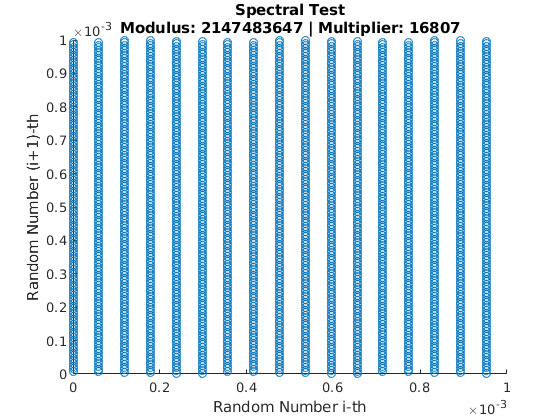
\includegraphics[width=\columnwidth]{fig/evaluation-randomness-spectral-16807}
	\caption{The Spectral Test to evaluate the randomness of the random number generator $(16807,2^{31}-1, 1)$ in the interval $(0, 10^{-3})$.}
	\label{fig:evaluation-randomness-spectral-16807}
\end{figure}

\begin{figure}
	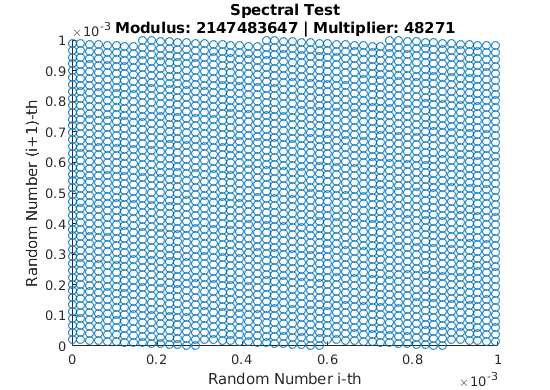
\includegraphics[width=\columnwidth]{fig/evaluation-randomness-spectral-48271}
	\caption{The Spectral Test to evaluate the randomness of the random number generator $(48271,2^{31}-1, 1)$ in the interval $(0, 10^{-3})$.}
	\label{fig:evaluation-randomness-spectral-48271}
\end{figure}

\begin{figure}
	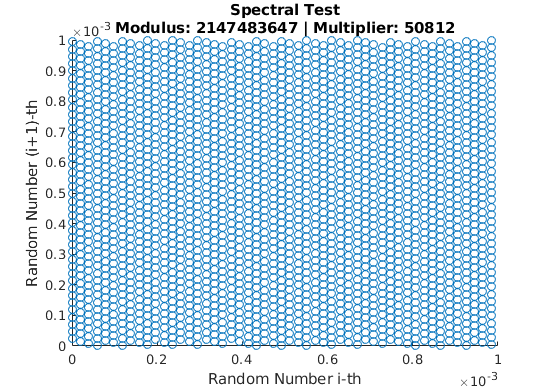
\includegraphics[width=\columnwidth]{fig/evaluation-randomness-spectral-50812}
	\caption{The Spectral Test to evaluate the randomness of the random number generator $(50812,2^{31}-1, 1)$ in the interval $(0, 10^{-3})$.}
	\label{fig:evaluation-randomness-spectral-50812}
\end{figure}

\begin{figure}
	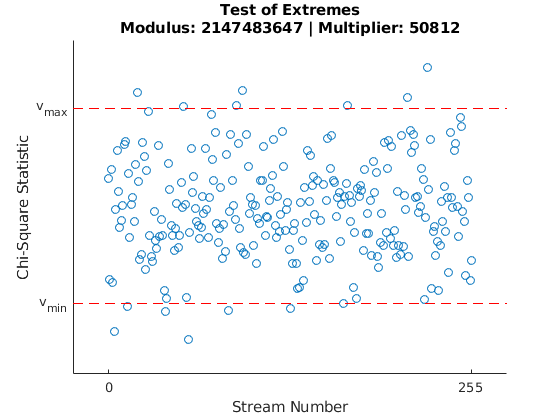
\includegraphics[width=\columnwidth]{fig/evaluation-randomness-extremes-50812}
	\caption{The Test of Extremes with $d=5$ to evaluate the randomness of the random number generator $(50812,2^{31}-1, 256)$.}
	\label{fig:evaluation-randomness-extremes-50812}
\end{figure}

\begin{figure}
	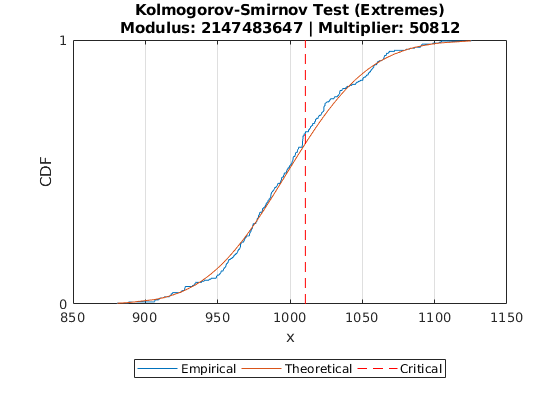
\includegraphics[width=\columnwidth]{fig/evaluation-randomness-kolmogorov-smirnov-50812}
	\caption{The Kolmogorov-Smirnov Analysis (leveraging the Test of Extremes with $d=5$) to evaluate the randomness of the random number generator $(50812,2^{31}-1, 256)$ with $0.95$ confidence level.}
	\label{fig:evaluation-randomness-kolmogorov-smirnov-50812}
\end{figure}


% %
% PERFORMANCE ANALYSIS
% %
\subsection{Performance Analysis}
Let us now consider the experimental results about system performance recorded by our simulator.
In all experiments we considered values stated in Section~\ref{sec:performance-modeling} with a preemption policy based on \textit{random selection}.

\subsection{Transient Analysis}
\label{sec:evaluation-transient-analysis}
First, we conduct a \textit{transient analysis} to evaluate the system stationary in order to (i) prove its convergence to the steady-state and (ii) estimate the duration of the transient period.
%
In fact, given a system that converges to stationary, the knowledge of the duration of the transient period is really important to conduct an effective performance evaluation. In particular, it allows the analyst to focus performance evaluation on a system in its stationary conditions.
%
In the transient analysis we focus on the global system throughput as it can be considered a good representation of the dependency of the system from the initial state.

The following results have been produced by considering an ensemble of $5$ replications, where the $i+1$-th replication is initialized with the last seed of the $i$-th replication, so as to achieve the best decoupling between random sequences of different replications.

In Figure \ref{fig:evaluation-transient-analysis-throughput} we show the transient analysis of the global throughput in the whole system.

The results show that the system reaches the steady-state.
This result is not surprising, because the presence of a stabilizing \textit{infinite-buffer centre}, i.e. the Cloud, largely compensates the possible instability of the \textit{thresholded finite-buffer centre}, i.e. the Cloudlet.

\begin{figure}
	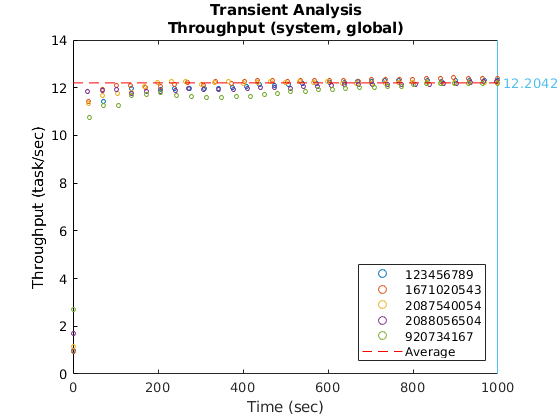
\includegraphics[width=\columnwidth]{fig/evaluation-transient-analysis-throughput}
	\caption{Transient analysis for global throughput in the whole system.}
	\label{fig:evaluation-transient-analysis-throughput}
\end{figure}


\subsection{Performance Evaluation}
Let us now focus on the \textit{performance evaluation}, taking into account the following metrics:

\begin{enumerate}
	\item \textit{response time} both global and classed, both for the system as a whole and for each subsystem;
	
	\item \textit{throughput} both global and classed, both for the system as a whole and for each subsystem;
	
	\item \textit{population} both global and classed, both for the system as a whole and for each subsystem;
	
	\item \textit{interrupted ratio} for tasks belonging to the $2^{nd}$ class.
	
	\item \textit{interrupted response time} for tasks belonging to the $2^{nd}$ class.
\end{enumerate}

In our experiment we assume $S=N=20$, $k=64$ batches, batch dimension $b=512$ and initial seed $iseed=123456789$.
%
Theoretical results have been computed using the formulas presented in Section~\ref{sec:performance-modeling}, assuming the experimentally computed value $E[T_{clt,2,lost}]=1.47445;s.$.

In Table

\begin{figure}
	\begin{center}
		\begin{tabular}{|c||c|c|}
			\hline
			Measure & Theoretical & Experimental\\
			\hline
			$a_{clt,1}$  & $0.978326334857105$ & $0.97911346521$ \\
			$a_{clt_2}$  & $0.603529764734761$ & $0.60502880468$ \\
			$r$          & $0.183573830264005$ & $0.15525744148$ \\	
			\hline
		\end{tabular}
	\end{center}
	\caption{Routing probabilities: comparison between the theoretical result, computed with the analytical model, and the experimental result, computed leveraging our simulator.}
	\label{tbl:evaluation-routing-probabilities}
\end{figure}

\begin{figure}
	\begin{center}
		\begin{tabular}{|c||c|c|}
			\hline
			Measure & Theoretical & Experimental\\
			\hline
			$E[N_{clt}]$  & $123456789$ & $123456789\pm 0.00342$ \\
			$E[N_{clt,1}]$  & $123456789$ & $123456789\pm 0.00342$ \\
			$E[N_{clt,2}]$  & $123456789$ & $123456789\pm 0.00342$ \\
			$E[T_{clt}]$  & $123456789$ & $123456789\pm 0.00342$ \\
			$E[T_{clt,1}]$  & $123456789$ & $123456789\pm 0.00342$ \\
			$E[T_{clt,2}]$  & $123456789$ & $123456789\pm 0.00342$ \\
			$X_{clt}$  & $123456789$ & $123456789\pm 0.00342$ \\
			$X_{clt,1}$  & $123456789$ & $123456789\pm 0.00342$ \\
			$X_{clt,2}$  & $123456789$ & $123456789\pm 0.00342$ \\
			\hline
			$E[N_{cld}]$  & $123456789$ & $123456789\pm 0.00342$ \\
			$E[N_{cld,1}]$  & $123456789$ & $123456789\pm 0.00342$ \\
			$E[N_{cld,2}]$  & $123456789$ & $123456789\pm 0.00342$ \\
			$E[T_{cld}]$  & $123456789$ & $123456789\pm 0.00342$ \\
			$E[T_{cld,1}]$  & $123456789$ & $123456789\pm 0.00342$ \\
			$E[T_{cld,2}]$  & $123456789$ & $123456789\pm 0.00342$ \\
			$X_{cld}$  & $123456789$ & $123456789\pm 0.00342$ \\
			$X_{cld,1}$  & $123456789$ & $123456789\pm 0.00342$ \\
			$X_{cld,2}$  & $123456789$ & $123456789\pm 0.00342$ \\
			\hline
			$E[N_{sys}]$  & $123456789$ & $123456789\pm 0.00342$ \\
			$E[N_{sys,1}]$  & $123456789$ & $123456789\pm 0.00342$ \\
			$E[N_{sys,2}]$  & $123456789$ & $123456789\pm 0.00342$ \\
			$E[T_{sys}]$  & $123456789$ & $123456789\pm 0.00342$ \\
			$E[T_{sys,1}]$  & $123456789$ & $123456789\pm 0.00342$ \\
			$E[T_{sys,2}]$  & $123456789$ & $123456789\pm 0.00342$ \\
			$X_{sys}$  & $123456789$ & $123456789\pm 0.00342$ \\
			$X_{sys,1}$  & $123456789$ & $123456789\pm 0.00342$ \\
			$X_{sys,2}$  & $123456789$ & $123456789\pm 0.00342$ \\
			\hline
			$E[T_{restarted}]$  & $123456789$ & $123456789\pm 0.00342$ \\
			$RestartRatio$  & $123456789$ & $123456789\pm 0.00342$ \\			
			\hline
		\end{tabular}
	\end{center}
	\caption{Performance metrics: comparison between the theoretical result, computed with the analytical model, and the experimental result with level of confidence $95\%$, computed leveraging our simulator.}
	\label{tbl:evaluation-performance-metrics}
\end{figure}

%%
% DISTRIBUTION ANALYSIS
%%
\subsection{Distribution Analysis}
\label{sec:evaluation-distribution-analysis}
In this Section we show the distribution analysis of the Cloudlet global throughput. 
In particular, we focus on both (i) the Probability Density Function (PDF) estimation leveraging distribution fitting, and (ii) the comparison between theoretical and experimental Cumulative Distribution Function (CDF).

In Figure~\ref{fig:evaluation-distribution-analysis-pdf-throughput-cloudlet-global} and  Figure~\ref{fig:evaluation-distribution-analysis-cdf-throughput-cloudlet-global} we show the PDF estimation and the CDF analysis, respectively, for the global Cloudlet throughput when $S=N=20$, where we adopted the \textit{Freedman-Diaconis Rule} for the binning schema.
Results show that the best fitting is the \textit{Normal Distribution} with parameters $\mu\approx7.403$ and $\sigma\approx0.364$.
%
The Normal behavior shown here can be considered as a further good proof of both the system stationary and the effectiveness of the batch means as a tool to study steady-state statistics.

\begin{figure}
	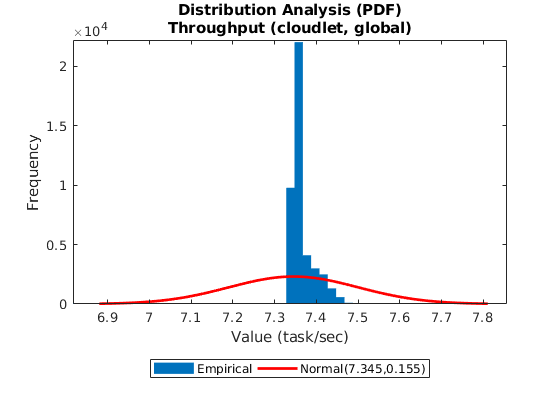
\includegraphics[width=\columnwidth]{fig/evaluation-distribution-analysis-pdf-throughput-cloudlet-global}
	\caption{Distribution analysis (Probability Distribution Function)for the Cloudlet global throughput with threshold $S=N=20$.}
	\label{fig:evaluation-distribution-analysis-pdf-throughput-cloudlet-global}
\end{figure}

\begin{figure}
	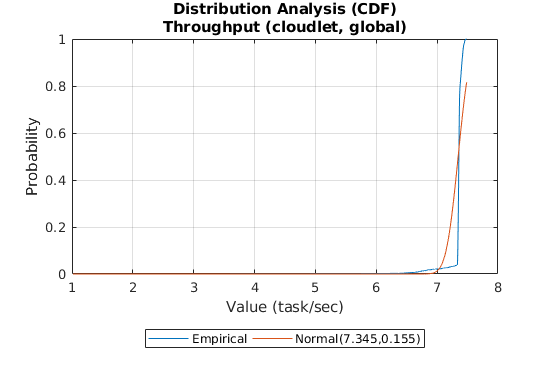
\includegraphics[width=\columnwidth]{fig/evaluation-distribution-analysis-cdf-throughput-cloudlet-global}
	\caption{Distribution analysis (Cumulative Distribution Function) for the Cloudlet global throughput with threshold $S=N=20$.}
	\label{fig:evaluation-distribution-analysis-cdf-throughput-cloudlet-global}
\end{figure}
\section{Usage}
\label{sec:usage}


In this Section we show how to configure and run experiments and some sample outputs to provide a better idea of what has been created.

The test of extremes for a custom random number generator produces the output shown in Figure~\ref{fig:usage-randomness-extremes} and can be executed with default configuration by running the script

\begin{lstlisting}
exp/random/randomness/extremes/main.py
\end{lstlisting}

\begin{figure}
	\centering
	\lstinputlisting{ext/randomness-extremes.txt}
	\caption{A sample output of the Test of Extremes.}
	\label{fig:usage-randomness-extremes}
\end{figure}

The test of Kolmogorov-Smirnov for a custom random number generator produces the output shown in Figure~\ref{fig:usage-randomness-kolmogorov-smirnov} and can be executed with default configuration by running the script

\begin{lstlisting}
exp/random/randomness/kolmogorov-smirnov/main.py
\end{lstlisting}

\begin{figure}
	\centering
	\lstinputlisting{ext/randomness-kolmogorov-smirnov.txt}
	\caption{A sample output of the Test of Kolmogorov-Smirnov.}
	\label{fig:usage-randomness-kolmogorov-smirnov}
\end{figure}

The simulation is configured providing a configuration YAML file as the one shown in Figure~\ref{fig:usage-simulation-configuration} and can be executed by running the script

\begin{lstlisting}
exp/simulation/performance/main.py
\end{lstlisting}

\begin{figure}
	\centering
	\lstinputlisting{ext/simulation-configuration.yaml}
	\caption{A sample configuration for a simulation experiment.}
	\label{fig:usage-simulation-configuration}
\end{figure}



\section{Conclusions}
\label{sec:conclusions}

\lipsum[1-3]


%*******************************************************************************
% Bibliography
%*******************************************************************************
\bibliographystyle{biblio}
\bibliography{./ref/biblio}

\end{document}
